% !TEX root = emba_2027_ouverture.tex
% Cas canadiens, d’après la fin de la séance 4. Les déplacements
% schématiques sont relatifs au scénario de référence, sans échelle empirique.
\newcommand{\sourceCas}[2][0pt]{\par\vspace{.18cm}{\raggedleft\scriptsize\color{black!65}%
  \raisebox{-#1}[\height][\depth]{#2}\par}}
\newcommand{\sourceTarifs}{\href{https://www.banqueducanada.ca/publication/rpm/rpm-2026-10-28/hypotheses-tarifaires/}{Banque du Canada, hypothèses tarifaires d’octobre 2026}}
\newcommand{\sourcePerspectives}{\href{https://www.banqueducanada.ca/publication/rpm/rpm-2026-10-28/perspectives-canadiennes/}{Banque du Canada, perspectives d’octobre 2026}}
\newcommand{\sourceIPC}{\href{https://www150.statcan.gc.ca/n1/daily-quotidien/261116/dq261116a-fra.htm}{Statistique Canada, IPC d’octobre 2026}}

\begin{frame}{Une inflation élevée malgré un PIB sous son potentiel}
  \begin{columns}[T,onlytextwidth]
    \begin{column}{.48\textwidth}
      \textbf{Écart de production}\par\vspace{4pt}
      {\LARGE\bfseries \textminus{}1,25\,\% à \textminus{}0,25\,\%}\par\vspace{4pt}
      {\small Fourchette estimée par la Banque du Canada au troisième trimestre de 2026.}
    \end{column}
    \begin{column}{.45\textwidth}
      \textbf{Inflation annuelle}\par\vspace{4pt}
      {\LARGE\bfseries 3,1\,\%}\par\vspace{4pt}
      {\small Hausse de l’IPC en octobre 2026. Hors énergie, elle était de 2,0\,\%.}
    \end{column}
  \end{columns}
  \vspace{.40cm}
  \begin{piedADAS}
    Quels chocs peuvent à la fois \textbf{freiner les ventes} et \textbf{comprimer les marges}\,?
  \end{piedADAS}
  \sourceCas{\href{https://www.banqueducanada.ca/publication/rpm/rpm-2026-10-28/conjoncture-canadienne/}{Banque du Canada, conjoncture d’octobre 2026}\quad\sourceIPC}
  \note{Demander aux participants quel choc isolé expliquerait une activité inférieure au potentiel
    et des pressions sur les prix. Un écart de production négatif et une inflation supérieure à la
    cible peuvent coexister. Les périodes et les mesures diffèrent. Un graphique AD-AS compare
    des niveaux de prix entre deux scénarios, alors que l’IPC mesure ici une variation sur douze mois.
    Pour la séance du 28 janvier, actualiser les deux chiffres et confronter le diagnostic à la
    décision et aux projections de la Banque du 27 janvier.}
\end{frame}

% Deux lectures de l’inflation.
\begin{frame}{Inflation globale et inflation fondamentale au Canada}
  \centering
  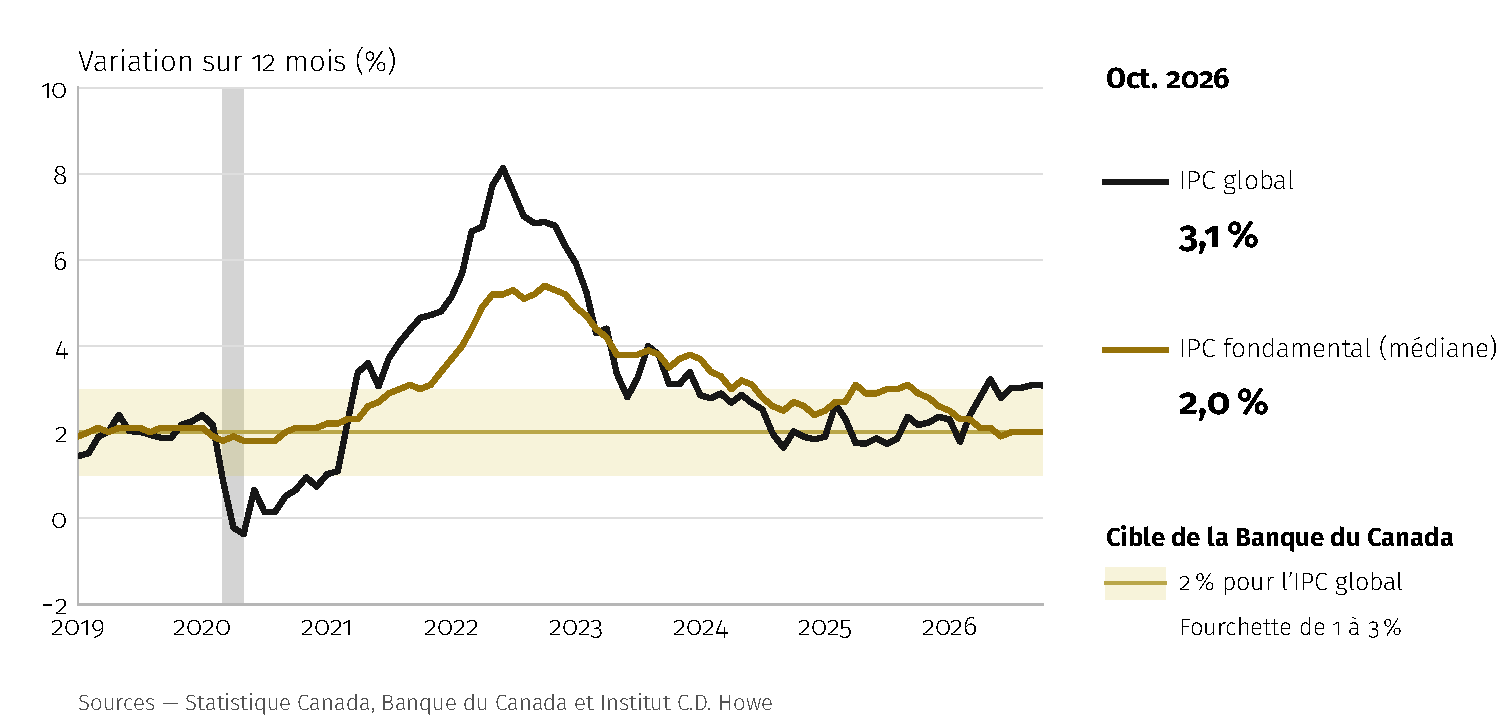
\includegraphics[width=\textwidth]{inflation_canada.pdf}
  \note{Le modèle indique un niveau de prix. Les courbes qui suivent mesurent sa variation
    sur douze mois. Si l’inflation ralentit tout en restant positive, le niveau de prix
    continue de monter. L’IPC global suit le prix du panier de consommation des ménages. L’IPC-médiane
    est une mesure de l’inflation fondamentale fondée sur la médiane pondérée des
    variations de prix. La cible de 2\,\% s’applique à l’inflation de l’IPC global.
    Si les deux mesures divergent, quelles hausses de prix jugez-vous assez persistantes
    pour les intégrer au budget de l’an prochain\,?}
\end{frame}

\begin{frame}{Prix à la production et à la consommation au Canada}
  \centering
  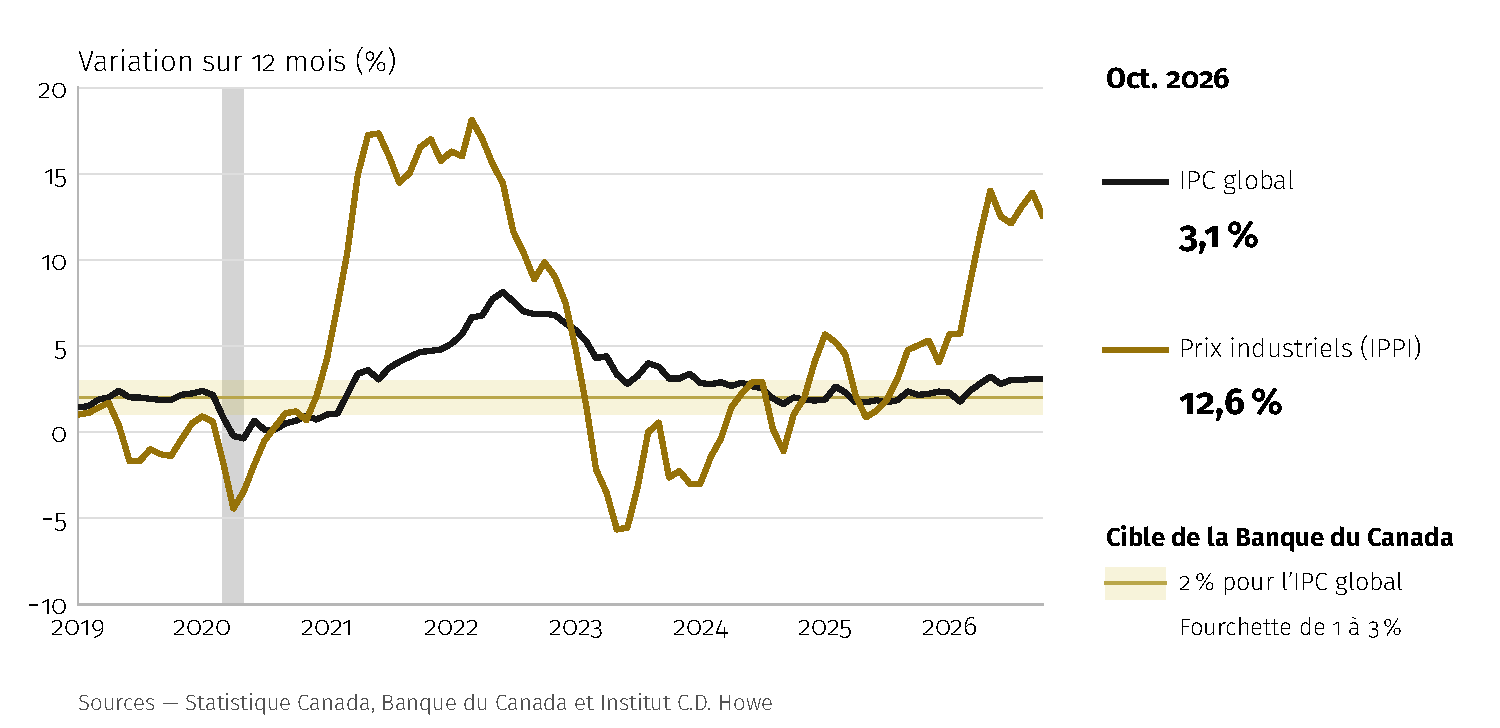
\includegraphics[width=\textwidth]{inflation_production_canada.pdf}
  \note{L’indice des prix des produits industriels (IPPI) mesure les prix que les
    fabricants canadiens reçoivent à la sortie de l’usine. Demander à un fabricant
    et à un détaillant quel indice se rapproche le plus de leurs prix de vente.
    Si les prix en usine augmentent plus vite que les prix à la consommation,
    de quoi dépend la capacité de répercuter la hausse sur les clients\,?}
\end{frame}

% Mettre le PIB observé en regard du potentiel estimé.
\begin{frame}{L’économie canadienne tourne-t-elle près de sa capacité\,?}
  \centering
  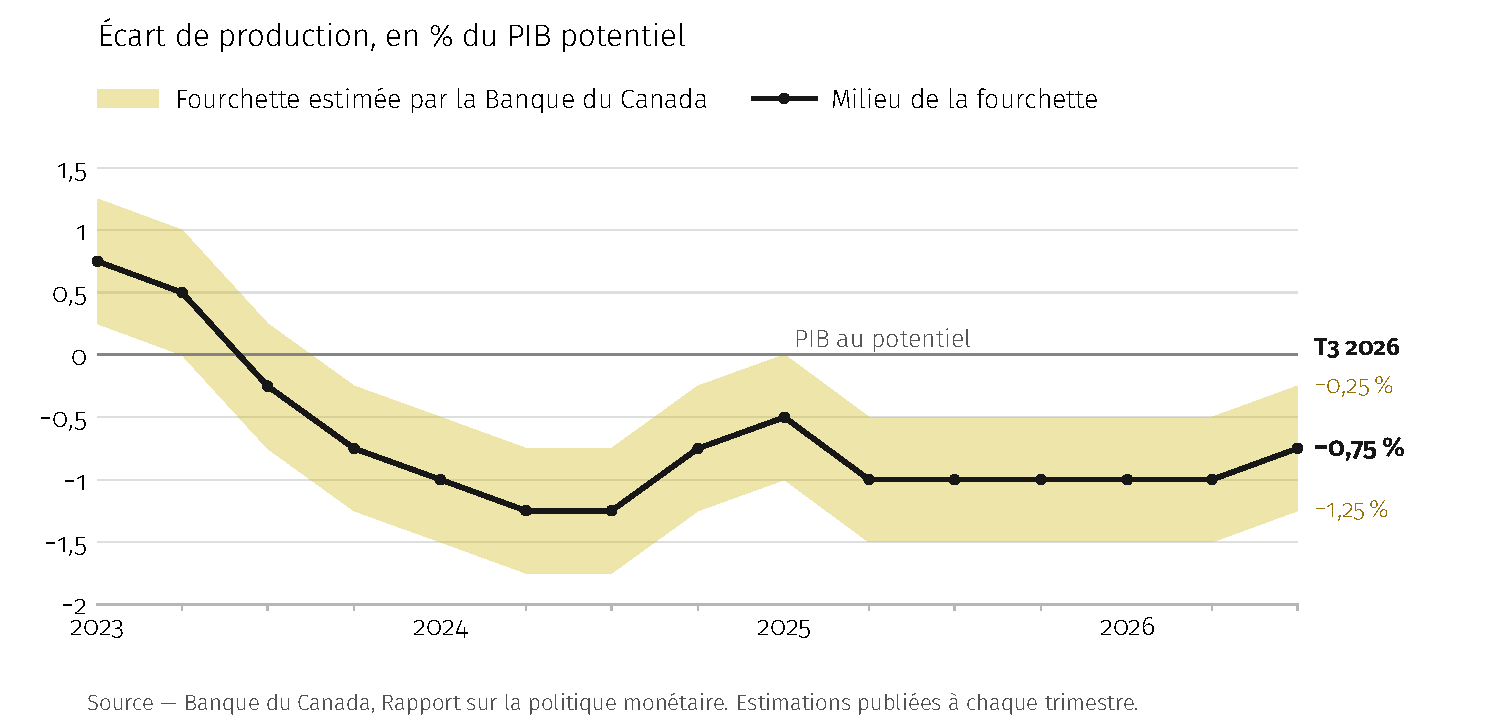
\includegraphics[width=\textwidth]{ecart_production_canada.pdf}
  \note{La bande dorée relie les bornes de la fourchette publiée par la Banque du Canada à chaque trimestre.
    Chaque point noir marque le milieu des deux bornes. La ligne grise à zéro correspond au PIB potentiel. Une fourchette
    entièrement sous zéro indique que la Banque estimait que l’économie disposait
    de capacités inutilisées. Le PIB peut donc augmenter pendant que l’écart reste
    négatif. Croiser cette estimation avec les prix et les composantes du PIB.
    Quels indices appuient l’hypothèse d’un recul de la demande ou celle d’une hausse
    des coûts\,? Revenir à l’évaluation du Rapport du 27 janvier. Si les commandes
    rebondissent, jusqu’où pouvez-vous augmenter la production avec vos équipements
    et vos équipes actuels\,? Quel signal vous ferait investir\,?}
\end{frame}

% Conjoncture et décision d’embauche.
\begin{frame}{Le marché du travail au Canada}
  \centering
  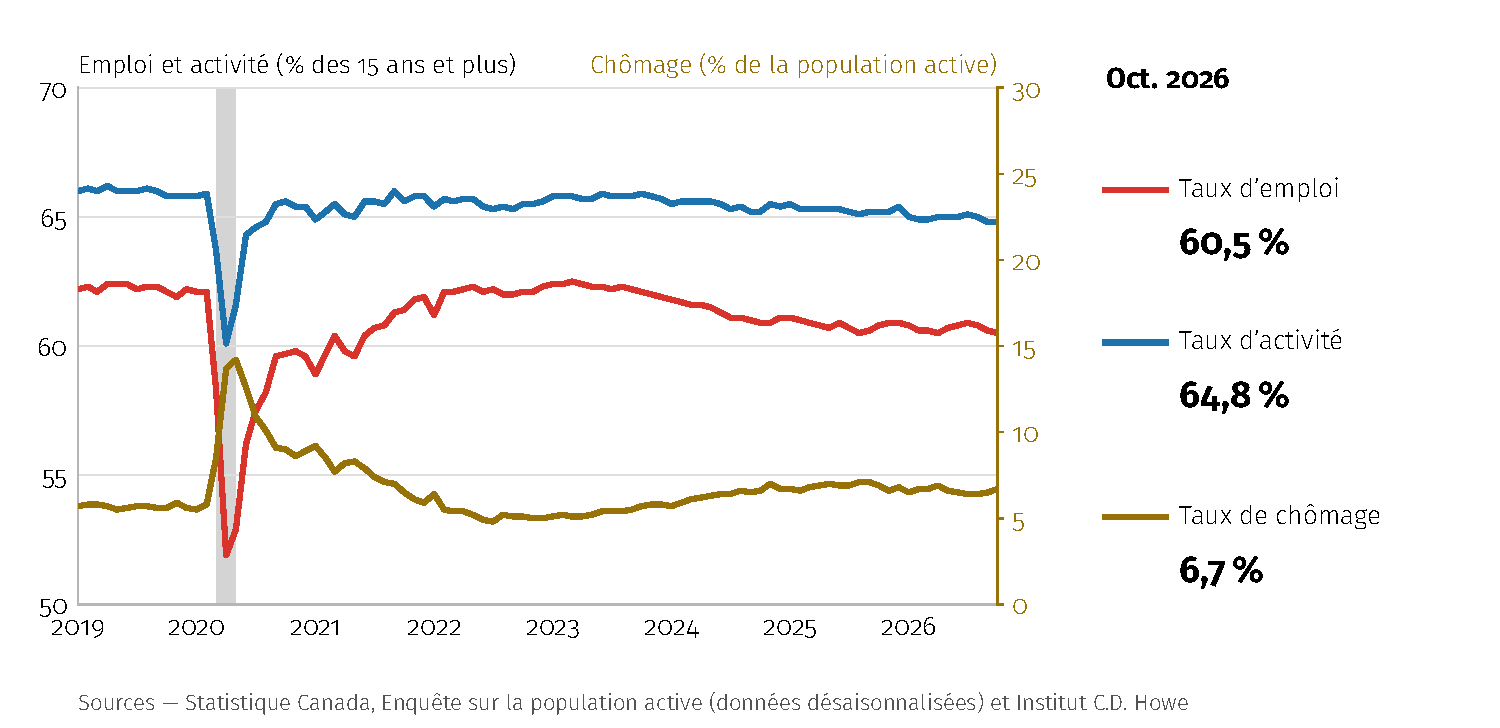
\includegraphics[width=\textwidth]{marche_travail_canada.pdf}
  \note{Le taux d’activité indique quelle part des personnes de 15 ans et plus occupent
    un emploi ou sont au chômage. Le taux d’emploi indique quelle part de cette même
    population occupe un emploi. Le taux de chômage rapporte le nombre de chômeurs à
    la population active. Comparer deux scénarios où le taux de chômage baisse :
    dans le premier, les entreprises embauchent davantage. Dans le second, des personnes
    qui cherchaient du travail quittent la population active. Quel scénario observez-vous
    dans votre région et votre métier\,? Vérifier le délai de recrutement et le nombre
    de candidatures qualifiées par poste avant de revoir le calendrier d’embauche.}
\end{frame}

% Les quatre cas AD-AS partagent le même repère, deux blocs de lecture et une ligne de source.
\newcommand{\casADAS}[6]{%
  \vspace*{.34cm}
  \begin{columns}[T,onlytextwidth]
    \begin{column}{.525\textwidth}
      \renewcommand{\hauteurAxePrixEMBA}{4.72}%
      \renewcommand{\hautCadreMarcheEMBA}{5.29}%
      \tikzset{unites marche/.append style={y=.86cm}}%
      \resizebox{\linewidth}{!}{#1}
    \end{column}
    \begin{column}{.445\textwidth}
      \raggedright\small
      \textbf{#2}\\[1pt]#3\par
      \vspace{7pt}
      \textcolor{offreEMBA}{\textbf{#4}}\\[1pt]#5
    \end{column}
  \end{columns}
  \begin{tikzpicture}[remember picture,overlay]
    \node[anchor=base east,inner sep=0pt,font=\scriptsize,text=black!65]
      at ([xshift=-1.2cm,yshift=.77cm]current page.south east) {#6};
  \end{tikzpicture}}

\begin{frame}[t]{Les droits de douane américains freinent la demande au Canada}
  \casADAS{\schemaADAS{demande}}
    {De 5,0\,\% à 7,5\,\%}
    {Droit américain moyen estimé sur les biens canadiens, de juillet à octobre 2026.}
    {Le canal des exportations}
    {Si les exportations reculent, AD se déplace vers la gauche. Un fabricant qui prévoit une baisse durable des commandes peut reporter l’agrandissement de son usine.}
    {\sourceTarifs}
  \note{Isoler l’effet des droits américains sur les achats de produits canadiens. À importations
    inchangées, le recul des exportations réduit les exportations nettes et déplace la demande
    agrégée vers la gauche. À offre agrégée inchangée, le PIB réel et le niveau des prix sont
    plus faibles à court terme que dans le scénario sans hausse des droits. Si les entreprises
    reportent leurs investissements, le recul de la demande agrégée s’accentue. Demander à un
    exportateur quel niveau de commandes fermes justifierait de relancer son projet d’agrandissement.}
\end{frame}

% Emploi sectoriel, d’après le graphique de la séance 1 du MBA.
\begin{frame}{L’emploi selon l’exposition aux droits de douane américains}
  \centering
  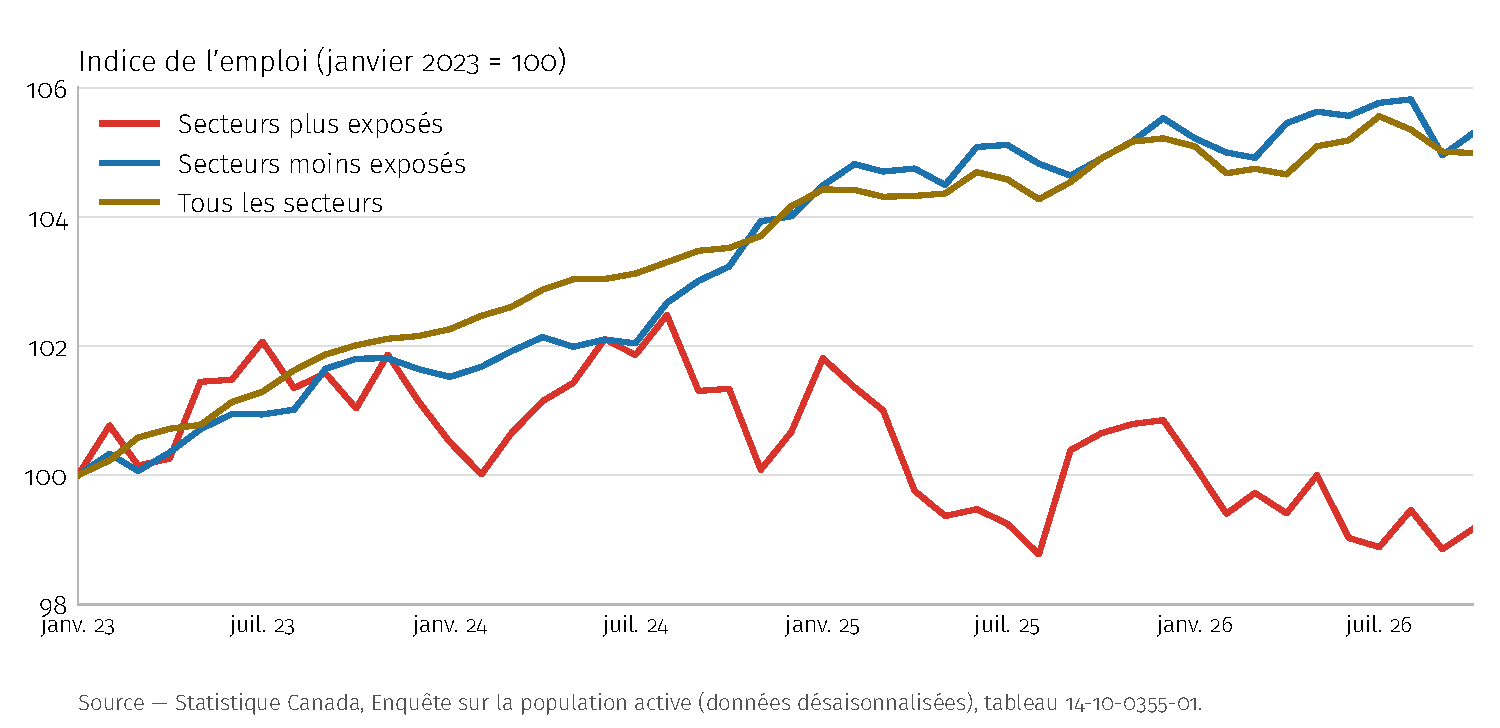
\includegraphics[width=\textwidth]{emploi_exposition_douane.pdf}
  \note{Les secteurs plus exposés regroupent la fabrication, l’agriculture, la foresterie,
    la pêche, les mines et l’extraction de pétrole et de gaz. Les secteurs moins exposés
    regroupent la santé et l’assistance sociale, l’enseignement, les administrations
    publiques, la construction, l’hébergement et la restauration, ainsi que le commerce
    de détail. La série nationale inclut aussi les secteurs absents des deux groupes.
    Chaque courbe rapporte l’emploi à son propre niveau de janvier 2023.
    Les écarts observés peuvent aussi refléter la demande intérieure ou les prix des
    matières premières. Avant d’ajuster vos effectifs, que vérifieriez-vous dans votre
    carnet de commandes américain\,?}
\end{frame}

\begin{frame}[t]{Le pétrole et les contre-tarifs renchérissent les intrants}
  \casADAS{\schemaADAS{offre}}
    {Transport et fabrication}
    {En octobre 2026, l’essence coûte 30,9\,\% de plus qu’un an plus tôt. Les contre-tarifs canadiens rendent les intrants américains plus chers.}
    {À prix de vente donné}
    {Produire rapporte moins. L’offre agrégée recule à court terme.}
    {\sourceIPC\quad\sourceTarifs}
  \note{La perturbation de l’offre mondiale de pétrole et les marges de raffinage élevées
    ont accru les coûts de l’énergie. La variation annuelle du prix de l’essence comprend aussi
    un effet de base. Les contre-tarifs touchent notamment l’acier et l’aluminium.
    Ce graphique isole les coûts. Le Canada exporte aussi du pétrole. Un producteur canadien
    peut recevoir un prix plus élevé alors qu’un transporteur paie son carburant plus cher.
    Quel contrat permet de réviser la surcharge de carburant, et à quelle date\,?}
\end{frame}

\begin{frame}{Le coût des matières brutes pour les fabricants canadiens}
  \centering
  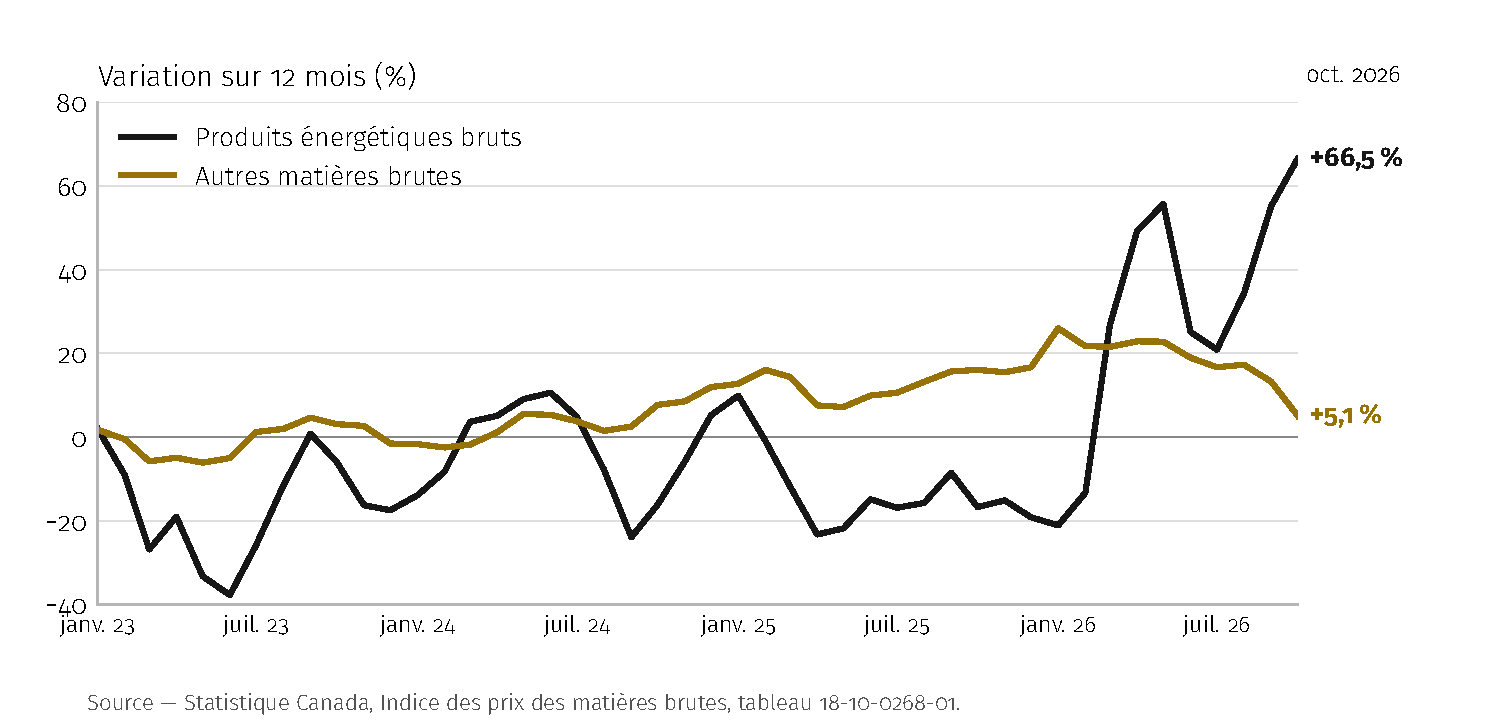
\includegraphics[width=\textwidth]{prix_matieres_brutes.pdf}
  \note{L’IPMB mesure les prix d’achat des matières brutes par les fabricants canadiens.
    Les produits énergétiques bruts comprennent notamment le pétrole brut, le gaz naturel et le charbon.
    En octobre 2026, leurs prix dépassent de 66,5\,\% leur niveau d’un an plus tôt, contre 5,1\,\%
    pour les autres matières brutes. Ces séries ne permettent pas d’isoler l’effet des contre-tarifs.
    Dans votre secteur, quelle part des achats est exposée à l’énergie et à quelle échéance
    pouvez-vous renégocier vos prix de vente\,?}
\end{frame}

% Deux étapes du même cas, dans le repère du rappel AD-AS. À l’impact,
% le choc de coûts domine l’effet désinflationniste de la demande dans cet exemple.
\newcommand{\trajectoireCanada}[1]{%
  \begin{tikzpicture}[unites marche,font=\footnotesize,
    courbe/.style={line width=1.15pt,line cap=round},
    guide/.style={black!28,thin},
    deplacement/.style={shiftarrow,shorten <=3.5pt,shorten >=3.5pt}]
    \repereMarcheEMBA
    \coordinate (adG) at (0,3.8); \coordinate (adD) at (5.5,.5);
    \coordinate (adBasG) at (0,3.2); \coordinate (adBasD) at (4.5,.5);
    \coordinate (asG) at (0,.2); \coordinate (asD) at (5.5,3.5);
    \coordinate (asHautG) at (0,1.5); \coordinate (asHautD) at (4,3.9);
    \coordinate (E0) at (intersection of adG--adD and asG--asD);
    \coordinate (E1) at (intersection of adBasG--adBasD and asHautG--asHautD);
    \ifstrequal{#1}{reprise}{%
      \coordinate (adRepriseG) at ($(adBasG)+(0,1.2)$);
      \coordinate (adRepriseD) at ($(adRepriseG)+(adD)-(adG)$);
      \coordinate (E2) at (intersection of adRepriseG--adRepriseD and asHautG--asHautD);
    }{}
    \draw[black!55,line width=.7pt] (E0 |- O) node[below,text=black] {$Y_{\text{pot}}$}
      -- (E0 |- axePrix) node[above right,inner xsep=0pt,text=black!75] {PIB potentiel};
    \draw[guide] (O |- E1) node[left,text=black] {$P_1$} -- (E1)
      -- (E1 |- O) node[below,text=black] {$Y_1$};
    \ifstrequal{#1}{impact}{%
      \draw[guide] (O |- E0) node[left,text=black] {$P_0$} -- (E0);
      \draw[courbe,courbeInitialeEMBA] (asG) -- (asD) node[right,curvelabel,text=black!50] {AS$_0$};
      \draw[courbe,courbeInitialeEMBA] (adG) -- (adD) node[right,curvelabel,text=black!50] {AD$_0$};
      \draw[courbe] (adBasG) -- (adBasD) node[right,curvelabel] {AD$_1$};
      \draw[deplacement] (4.7,.98) -- (3.7,.98);
      \draw[deplacement,offreEMBA] (4.85,3.11) -- ({4.85 - 1.3 / .6},3.11);
      \filldraw[fill=white] (E0) circle (2.4pt);
    }{%
      \draw[guide] (O |- E2) node[left,text=black] {$P_2$} -- (E2)
        -- (E2 |- O) node[below,text=black] {$Y_2$};
      \draw[courbe,courbeInitialeEMBA] (adBasG) -- (adBasD) node[right,curvelabel,text=black!50] {AD$_1$};
      \draw[courbe] (adRepriseG) -- (adRepriseD) node[right,curvelabel] {AD$_2$};
      \coordinate (repereG) at (0,1.28); \coordinate (repereD) at (6,1.28);
      \draw[deplacement] (intersection of adBasG--adBasD and repereG--repereD)
        -- (intersection of adRepriseG--adRepriseD and repereG--repereD);
    }
    \draw[courbe,offreEMBA] (asHautG) -- (asHautD) node[right,curvelabel] {AS$_1$};
    \ifstrequal{#1}{impact}{\fill (E1) circle (2.6pt);}{%
      \filldraw[fill=white] (E1) circle (2.4pt); \fill (E2) circle (2.6pt);}
    \draw[econaxis] (O) -- (axeQuantite) node[below left] {PIB réel};
    \draw[econaxis] (O) -- (axePrix) node[anchor=south west,inner xsep=0pt] {Niveau des prix};
  \end{tikzpicture}}

\begin{frame}[t]{Que se passe-t-il quand les deux chocs se cumulent\,?}
  \casADAS{\trajectoireCanada{impact}}
    {La production recule}
    {Les commandes à l’exportation diminuent et les coûts augmentent. Les deux chocs freinent le PIB réel.}
    {Quel effet sur les prix\,?}
    {Ici, le choc de coûts domine. Les prix montent malgré les capacités inutilisées.}
    {Scénario illustratif à partir du \href{https://www.banqueducanada.ca/publication/rpm/rpm-2026-10-28/conjoncture-canadienne/}{Rapport sur la politique monétaire d’octobre 2026}}
  \note{Comparer le cercle blanc et le point noir. Si le recul de la demande était plus
    fort, le niveau des prix pourrait baisser. Les déplacements ne sont pas calibrés et
    le PIB potentiel est tenu fixe à l’impact. Une hausse ponctuelle du niveau des prix
    accroît temporairement l’inflation. Pour juger de sa persistance, suivre les prix
    hors énergie, les salaires et les anticipations.}
\end{frame}

\begingroup
\newcommand{\rubriquepresse}[1]{%
  \noindent{\small\bfseries #1}\enspace{\color{EMBAor}\hrulefill}\par\vspace{2pt}}
% Bandeaux des trois journaux régionaux et marques de Québecor, d’après leurs sites.
% Pour la dépêche traduite par Zonebourse, reprendre le logo de Reuters du cours.
\newcommand{\articlepresse}[4]{%
  \begin{column}{.48\textwidth}
    \raggedright
    \href{#1}{\raisebox{-.42\height}{\includegraphics[height=.48cm,width=2cm,keepaspectratio]{logos/#2.png}}}%
    \hfill{\scriptsize\color{black!65}#4}\par\vspace{3pt}
    {\footnotesize\href{#1}{#3}\par}
  \end{column}}
\begin{frame}{L’investissement au Canada dans les manchettes}
  \rubriquepresse{Mégadéduction à la productivité}
  \begin{columns}[T,onlytextwidth]
    \articlepresse{https://www.leclaireurprogres.ca/nouvelles-nationales/ottawa-entend-stimuler-les-investissements-grace-a-de-nouveaux-avantages-fiscaux/}
      {eclaireur_progres}
      {Ottawa entend stimuler les investissements grâce à de nouveaux avantages fiscaux}
      {La Presse Canadienne · 15 sept. 2026}
    \articlepresse{https://www.tvanouvelles.ca/2026/11/05/megadeduction-a-la-productivite-un-cadeau-fiscal-de-36-g-aux-entreprises}
      {tva_nouvelles}
      {«\,Mégadéduction à la productivité\,»\,: un cadeau fiscal de 36~G\$ aux entreprises}
      {5 nov. 2026}
  \end{columns}
  \vspace{.17cm}
  \rubriquepresse{Investissements pétroliers}
  \begin{columns}[T,onlytextwidth]
    \articlepresse{https://ch.zonebourse.com/actualite-bourse/imperial-oil-depasse-les-previsions-de-benefice-grace-a-la-amelioration-des-marges-de-raffinage-ce785fdbdd8ef025}
      {reuters_source}
      {Imperial Oil envisage d’avancer le projet de sables bitumineux Aspen}
      {Zonebourse · 30 oct. 2026}
    \articlepresse{https://www.courrierfrontenac.qc.ca/nouvelles-nationales/le-projet-petrolier-bay-du-nord-franchit-le-dernier-obstacle-reglementaire/}
      {courrier_frontenac}
      {Le projet pétrolier Bay du Nord franchit le dernier obstacle réglementaire}
      {La Presse Canadienne · 21 nov. 2026}
  \end{columns}
  \vspace{.17cm}
  \rubriquepresse{Centres de données}
  \begin{columns}[T,onlytextwidth]
    \articlepresse{https://www.journaldequebec.com/2026/03/05/la-caisse-de-depot-aide-une-firme-americaine-a-construire-un-centre-de-donnees-a-montreal}
      {journal_de_quebec}
      {La Caisse de dépôt a aidé une firme américaine à construire un centre de données à Montréal}
      {5 mars 2026}
    \articlepresse{https://www.lhebdojournal.com/nouvelles-nationales/bell-agrandira-son-centre-de-donnees-consacre-a-lia-en-saskatchewan/}
      {hebdo_journal}
      {Bell agrandira son centre de données consacré à l’IA en Saskatchewan}
      {La Presse Canadienne · 14 sept. 2026}
  \end{columns}
  \note{Demander aux équipes de choisir une manchette. Quel signal leur ferait inscrire le projet
    dans leur carnet de commandes pour 2027\,? La mégadéduction permet de déduire immédiatement
    les dépenses admissibles. Les 36~G\$ représentent un allègement fiscal estimé sur cinq ans.
    Pour Aspen, Imperial envisage de devancer sa décision finale. Pour Bay du Nord, le plan de
    développement a reçu son autorisation réglementaire. Pour le projet de Bell, chercher à quel
    moment une tranche annoncée devient un chantier. Relier les achats d’équipement et les
    travaux effectivement réalisés à la composante investissement de la demande agrégée.}
\end{frame}
\endgroup

\begin{frame}[t]{En 2027, l’investissement pourrait relancer la demande}
  \casADAS{\trajectoireCanada{reprise}}
    {Pourquoi avancer un projet\,?}
    {Un pétrole durablement cher favorise certains projets énergétiques. La Mégadéduction à la productivité réduit le coût après impôt des projets admissibles.}
    {Si les investissements se réalisent}
    {La demande se redresse. À coûts inchangés, le PIB se rapproche de son potentiel.}
    {Scénario illustratif · \sourcePerspectives}
  \note{Reprendre le point d’arrivée des chocs de coûts et de demande. On maintient AS
    fixe pour isoler l’effet des dépenses d’investissement sur AD. À coût de financement donné, un rendement après impôt plus élevé rend davantage de projets rentables. Les capacités nouvelles peuvent accroître
    le PIB potentiel plus tard. Comparer deux scénarios pour janvier. Si les intentions
    se traduisent en commandes fermes, faut-il réserver de la capacité\,? Si les projets
    restent en attente, quelle dépense peut-on différer\,?}
\end{frame}
